\section{多模态计算}

\subsection{英文论文}
关键词为多模态计算的英文论文。IEEE Xpolre中选ADVANCED SEARCH然后在Search term中输入Multimodal computing。

\begin{figure}[H]
    \centering
    \begin{subfigure}{0.8\textwidth}
        \centering
        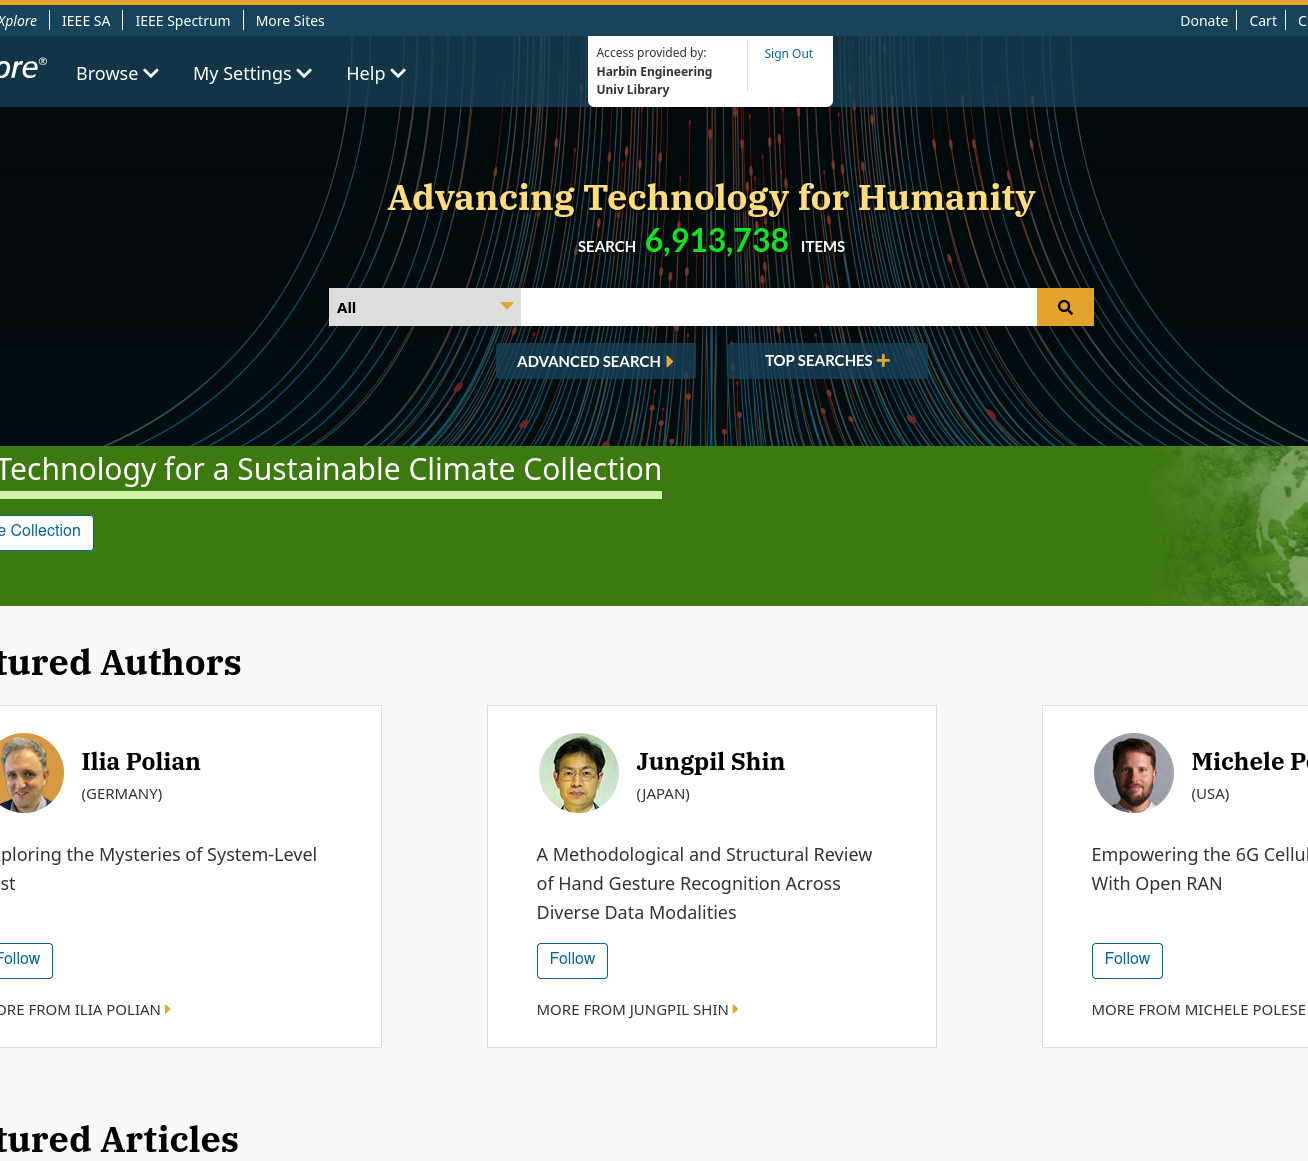
\includegraphics[width=0.7\textwidth]{./asserts/ieee_xpolre.png}
        \caption{IEEE Xpolre}
    \end{subfigure}

    % \hfill

    \begin{subfigure}{0.8\textwidth}
        \centering
        
\includegraphics[width=0.7\textwidth]{./asserts/en_search_multi_modal.png}
        \caption{Advanced search}
    \end{subfigure}
\end{figure}


\begin{itemize}
    \item 论文名:MMGT: MULTIMODAL GRAPH-BASED TRANSFORMER FOR PAIN DETECTION。
    \item 作者信息:
        \begin{enumerate}
            \item Kevin Feghoul:
                \begin{itemize}
                    \item Univ. Lille, Inserm, CHU Lille, UMR-S1172 LilNCog, Lille, France
                    \item Univ. Lille, CNRS, Centrale Lille, UMR 9189 CRIStAL, Lille, France 
                \end{itemize}
            \item Deise Santana Maia:
                \begin{itemize}
                    \item Univ. Lille, CNRS, Centrale Lille, UMR 9189 CRIStAL, Lille, France
                \end{itemize}

            \item Mohamed Daoudi:
                \begin{itemize}
                    \item Univ. Lille, CNRS, Centrale Lille, UMR 9189 CRIStAL, Lille, France
                    \item Centre for Digital Systems, IMT Nord Europe, Institut Mines-Télécom, Lille, France
                \end{itemize}

            \item Ali Amad:
                \begin{itemize}
                    \item Univ. Lille, Inserm, CHU Lille, UMR-S1172 LilNCog, Lille, France
                \end{itemize}
        \end{enumerate}

    \item 收录情况:
        \begin{itemize}
            \item Published in: 2023 31st European Signal Processing Conference (EUSIPCO)
            \item DOI: 10.23919/EUSIPCO58844.2023.10290098
        \end{itemize}

    \item 影响因子:会议论文,没有影响因子
    \item 被引情况:
        \begin{itemize}
            \item Kevin Feghoul, Deise Santana Maia, Mehdi El Amrani, Mohamed Daoudi, Ali Amad, "MGRFormer: A Multimodal Transformer Approach for Surgical Gesture Recognition", 2024 IEEE 18th International Conference on Automatic Face and Gesture Recognition (FG), pp.1-10, 2024.
        \end{itemize}
\end{itemize}



\subsection{中文}
关键词为多模态计算的中文论文
